\chapter{Going 3D: The PDB module}
\label{chapter:pdb}

Bio.PDB is a Biopython module that focuses on working with crystal structures of biological macromolecules. Among other things, Bio.PDB includes a PDBParser class that produces a Structure object, which can be used to access the atomic data in the file in a convenient manner. There is limited support for parsing the information contained in the PDB header. PDB file format is no longer being modified or extended to support new content and PDBx/mmCIF became the standard PDB archive format in 2014. All the Worldwide Protein Data Bank (wwPDB) sites uses the macromolecular Crystallographic Information File (mmCIF) data dictionaries to describe the information content of PDB entries. mmCIF uses a flexible and extensible key-value pair format for representing macromolecular structural data and imposes no limitations for the number of atoms, residues or chains that can be represented in a single PDB entry (no split entries!).

%Note the \verb|Bio.PDB| module requires Numerical Python (numpy) to be installed.

\section{Reading and writing crystal structure files}

\subsection{Reading an mmCIF file}

First create an \texttt{MMCIFParser} object:

\begin{minted}{pycon}
>>> from Bio.PDB.MMCIFParser import MMCIFParser
>>> parser = MMCIFParser()
\end{minted}
Then use this parser to create a structure object from the mmCIF file:
\begin{minted}{pycon}
>>> structure = parser.get_structure("1fat", "1fat.cif")
\end{minted}

To have some more low level access to an mmCIF file, you can use the \verb+MMCIF2Dict+ class to create a Python dictionary that maps all mmCIF
tags in an mmCIF file to their values. Whether there are multiple values
(like in the case of tag \verb+_atom_site.Cartn_y+, which holds
the $y$ coordinates of all atoms) or a single value (like the initial deposition date), the tag is mapped to a list of values.
The dictionary is created from the mmCIF file as follows:

\begin{minted}{pycon}
>>> from Bio.PDB.MMCIF2Dict import MMCIF2Dict
>>> mmcif_dict = MMCIF2Dict("1FAT.cif")
\end{minted}

Example: get the solvent content from an mmCIF file:
\begin{minted}{pycon}
>>> sc = mmcif_dict["_exptl_crystal.density_percent_sol"]
\end{minted}

Example: get the list of the $y$ coordinates of all atoms
\begin{minted}{pycon}
>>> y_list = mmcif_dict["_atom_site.Cartn_y"]
\end{minted}


\subsection{Reading files in the MMTF format}

You can use the direct MMTFParser to read a structure from a file:
%want to use doctest ../Tests lib:mmtf
%but will trigger PDBConstructionWarning
\begin{minted}{pycon}
>>> from Bio.PDB.mmtf import MMTFParser
>>> structure = MMTFParser.get_structure("PDB/4CUP.mmtf")
\end{minted}

Or you can use the same class to get a structure by its PDB ID:
%want online doctest here
\begin{minted}{pycon}
>>> structure = MMTFParser.get_structure_from_url("4CUP")
\end{minted}

This gives you a Structure object as if read from a PDB or mmCIF file.

You can also have access to the underlying data using the external
MMTF library which Biopython is using internally:
%want online doctest here
\begin{minted}{pycon}
>>> from mmtf import fetch
>>> decoded_data = fetch("4CUP")
\end{minted}
For example you can access just the X-coordinate.
\begin{minted}{pycon}
>>> print(decoded_data.x_coord_list)
\end{minted}

\subsection{Reading a PDB file}

First we create a \texttt{PDBParser} object:

\begin{minted}{pycon}
>>> from Bio.PDB.PDBParser import PDBParser
>>> parser = PDBParser(PERMISSIVE=1)
\end{minted}

The \texttt{PERMISSIVE} flag indicates that a number of common problems (see \ref{sec:problem_structures}) associated with PDB files will be ignored (but note that some atoms and/or residues will be missing). If the flag is not present a \texttt{PDBConstructionException} will be generated if any problems are detected during the parse operation.

The Structure object is then produced by letting the \texttt{PDBParser} object parse a PDB file (the PDB file in this case is called \verb|pdb1fat.ent|, \verb|1fat| is a user defined name for the structure):

\begin{minted}{pycon}
>>> structure_id = "1fat"
>>> filename = "pdb1fat.ent"
>>> structure = parser.get_structure(structure_id, filename)
\end{minted}

You can extract the header and trailer (simple lists of strings) of the PDB
file from the PDBParser object with the \texttt{get\_header} and \texttt{get\_trailer}
methods.  Note however that many PDB files contain headers with
incomplete or erroneous information. Many of the errors have been
fixed in the equivalent mmCIF files. \emph{Hence, if you are interested
in the header information, it is a good idea to extract information
from mmCIF files using the} \texttt{\emph{MMCIF2Dict}} \emph{tool
described above, instead of parsing the PDB header. }

Now that is clarified, let's return to parsing the PDB header. The
structure object has an attribute called \texttt{header} which is
a Python dictionary that maps header records to their values.

Example:

\begin{minted}{pycon}
>>> resolution = structure.header["resolution"]
>>> keywords = structure.header["keywords"]
\end{minted}
The available keys are \verb+name+, \verb+head+, \verb+deposition_date+, 
\verb+release_date+, \verb+structure_method+, \verb+resolution+, 
\verb+structure_reference+ (which maps to a list of references),
\verb+journal_reference+, \verb+author+, \verb+compound+ (which maps to
a dictionary with various information about the crystallized compound),
\verb+has_missing_residues+, \verb+missing_residues+, and \verb+astral+ 
(which maps to dictionary with additional information about the domain if present).

\verb+has_missing_residues+ maps to a bool that is True if at least
one non-empty \verb+REMARK 465+ header line was found. In this case
you should assume that the molecule used in the experiment has some 
residues for which no ATOM coordinates could be determined. 
\verb+missing_residues+ maps to a list of dictionaries with information
about the missing residues. \emph{The list of missing residues will be
empty or incomplete if the PDB header does not follow the template from
the PDB specification.}

The dictionary can also be created without creating a \texttt{Structure}
object, ie. directly from the PDB file:

\begin{minted}{pycon}
>>> from Bio.PDB import parse_pdb_header
>>> with open(filename, "r") as handle:
...     header_dict = parse_pdb_header(handle)
...
\end{minted}

\subsection{Reading a PQR file}

In order to parse a PQR file, proceed in a similar manner as in the case
of PDB files:

Create a \texttt{PDBParser} object, using the \texttt{is\_pqr} flag:

\begin{minted}{pycon}
>>> from Bio.PDB.PDBParser import PDBParser
>>> pqr_parser = PDBParser(PERMISSIVE=1, is_pqr=True)
\end{minted}

The \texttt{is\_pqr} flag set to \texttt{True} indicates that the file to be parsed is a PQR file, 
and that the parser should read the atomic charge and radius fields for each atom entry. Following the same procedure as for PQR files, a Structure object is then produced, and the PQR file is parsed.

\begin{minted}{pycon}
>>> structure_id = "1fat"
>>> filename = "pdb1fat.ent"
>>> structure = parser.get_structure(structure_id, filename, is_pqr=True)
\end{minted}

\subsection{Reading files in the PDB XML format}

That's not yet supported, but we are definitely planning to support that
in the future (it's not a lot of work). Contact the Biopython developers
via the mailing list if you need this.

\subsection{Writing mmCIF files}

The \texttt{MMCIFIO} class can be used to write structures to the mmCIF file format:

\begin{minted}{pycon}
>>> io = MMCIFIO()
>>> io.set_structure(s)
>>> io.save("out.cif")
\end{minted}
The \texttt{Select} class can be used in a similar way to \texttt{PDBIO} below.
mmCIF dictionaries read using \texttt{MMCIF2Dict} can also be written:

\begin{minted}{pycon}
>>> io = MMCIFIO()
>>> io.set_dict(d)
>>> io.save("out.cif")
\end{minted}

\subsection{Writing PDB files}

Use the \texttt{PDBIO} class for this. It's easy to write out specific parts
of a structure too, of course.

Example: saving a structure

\begin{minted}{pycon}
>>> io = PDBIO()
>>> io.set_structure(s)
>>> io.save("out.pdb")
\end{minted}
If you want to write out a part of the structure, make use of the
\texttt{Select} class (also in \texttt{PDBIO}). Select has four methods:

\begin{itemize}
\item \verb+accept_model(model)+
\item \verb+accept_chain(chain)+
\item \verb+accept_residue(residue)+
\item \verb+accept_atom(atom)+
\end{itemize}
By default, every method returns 1 (which means the model/\-chain/\-residue/\-atom
is included in the output). By subclassing \texttt{Select} and returning
0 when appropriate you can exclude models, chains, etc. from the output.
Cumbersome maybe, but very powerful. The following code only writes
out glycine residues:

\begin{minted}{pycon}
>>> class GlySelect(Select):
...     def accept_residue(self, residue):
...         if residue.get_name() == "GLY":
...             return True
...         else:
...             return False
...
>>> io = PDBIO()
>>> io.set_structure(s)
>>> io.save("gly_only.pdb", GlySelect())
\end{minted}
If this is all too complicated for you, the \texttt{Dice} module contains
a handy \texttt{extract} function that writes out all residues in
a chain between a start and end residue.

\subsection{Writing PQR files}

Use the \texttt{PDBIO} class as you would for a PDB file, with the flag \texttt{is\_pqr=True}. 
The PDBIO methods can be used in the case of PQR files as well.

Example: writing a PQR file

\begin{minted}{pycon}
>>> io = PDBIO(is_pqr=True)
>>> io.set_structure(s)
>>> io.save("out.pdb")
\end{minted}

\subsection{Writing MMTF files}

To write structures to the MMTF file format:

\begin{minted}{pycon}
>>> from Bio.PDB.mmtf import MMTFIO
>>> io = MMTFIO()
>>> io.set_structure(s)
>>> io.save("out.mmtf")
\end{minted}

The \texttt{Select} class can be used as above. Note that the bonding
information, secondary structure assignment and some other information contained
in standard MMTF files is not written out as it is not easy to determine from
the structure object. In addition, molecules that are grouped into the same
entity in standard MMTF files are treated as separate entities by
\texttt{MMTFIO}.


\section{Structure representation}

The overall layout of a \texttt{Structure} object follows the so-called SMCRA
(Structure/Model/Chain/Residue/Atom) architecture:

\begin{itemize}
\item A structure consists of models
\item A model consists of chains
\item A chain consists of residues
\item A residue consists of atoms
\end{itemize}
This is the way many structural biologists/bioinformaticians think
about structure, and provides a simple but efficient way to deal with
structure. Additional stuff is essentially added when needed. A UML
diagram of the \texttt{Structure} object (forget about the \texttt{Disordered}
classes for now) is shown in Fig. \ref{fig:smcra}. Such a data structure is not
necessarily best suited for the representation of the macromolecular content of
a structure, but it is absolutely necessary for a good interpretation of the
data present in a file that describes the structure (typically a PDB or MMCIF
file). If this hierarchy cannot represent the contents of a structure file, it
is fairly certain that the file contains an error or at least does not describe
the structure unambiguously. If a SMCRA data structure cannot be generated,
there is reason to suspect a problem. Parsing a PDB file can thus be used to
detect likely problems. We will give several examples of this in section
\ref{sec:problem_structures}.

\begin{figure}[htbp]
\begin{htmlonly}
\imgsrc[width=650, height=750]{images/smcra.png}
\end{htmlonly}
\begin{latexonly}
\centering
\includegraphics[width=0.8\textwidth]{images/smcra.png}
\end{latexonly}
\caption{UML diagram of SMCRA architecture of the \texttt{Structure} class used to represent a macromolecular structure.
Full lines with diamonds denote aggregation, full lines with
arrows denote referencing, full lines with triangles denote inheritance
and dashed lines with triangles denote interface realization.}
\label{fig:smcra}
\end{figure}

Structure, Model, Chain and Residue are all subclasses of the Entity base class.
The Atom class only (partly) implements the Entity interface (because an Atom
does not have children).

For each Entity subclass, you can extract a child by using a unique id for that
child as a key (e.g. you can extract an Atom object from a Residue object by
using an atom name string as a key, you can extract a Chain object from a Model
object by using its chain identifier as a key).

Disordered atoms and residues are represented by DisorderedAtom and DisorderedResidue
classes, which are both subclasses of the DisorderedEntityWrapper base class.
They hide the complexity associated with disorder and behave exactly as Atom
and Residue objects.

In general, a child Entity object (i.e. Atom, Residue, Chain, Model) can be
extracted from its parent (i.e. Residue, Chain, Model, Structure, respectively)
by using an id as a key.

\begin{minted}{pycon}
>>> child_entity = parent_entity[child_id]
\end{minted}

You can also get a list of all child Entities of a parent Entity object. Note
that this list is sorted in a specific way (e.g. according to chain identifier
for Chain objects in a Model object).

\begin{minted}{pycon}
>>> child_list = parent_entity.get_list()
\end{minted}

You can also get the parent from a child:
\begin{minted}{pycon}
>>> parent_entity = child_entity.get_parent()
\end{minted}

At all levels of the SMCRA hierarchy, you can also extract a \emph{full id}.
The full id is a tuple containing all id's starting from the top object (Structure)
down to the current object. A full id for a Residue object e.g. is something
like:

\begin{minted}{pycon}
>>> full_id = residue.get_full_id()
>>> print(full_id)
("1abc", 0, "A", ("", 10, "A"))
\end{minted}

This corresponds to:

\begin{itemize}
\item The Structure with id \verb|"1abc"|
\item The Model with id \verb|0|
\item The Chain with id \verb|"A"|
\item The Residue with id \verb|("", 10, "A")|
\end{itemize}
The Residue id indicates that the residue is not a hetero-residue (nor a water)
because it has a blank hetero field, that its sequence identifier is 10 and
that its insertion code is \verb|"A"|.

To get the entity's id, use the \verb+get_id+ method:
\begin{minted}{pycon}
>>> entity.get_id()
\end{minted}
You can check if the entity has a child with a given id by using the \verb+has_id+ method:
\begin{minted}{pycon}
>>> entity.has_id(entity_id)
\end{minted}
The length of an entity is equal to its number of children:
\begin{minted}{pycon}
>>> nr_children = len(entity)
\end{minted}

It is possible to delete, rename, add, etc. child entities from a parent entity,
but this does not include any sanity checks (e.g. it is possible to add two
residues with the same id to one chain). This really should be done via a nice
Decorator class that includes integrity checking, but you can take a look at
the code (Entity.py) if you want to use the raw interface.

\subsection{Structure}

The Structure object is at the top of the hierarchy. Its id is a user given
string. The Structure contains a number of Model children. Most crystal structures
(but not all) contain a single model, while NMR structures typically consist
of several models. Disorder in crystal structures of large parts of molecules
can also result in several models.

\subsection{Model}

The id of the Model object is an integer, which is derived from the position
of the model in the parsed file (they are automatically numbered starting from
0).
Crystal structures generally have only one model (with id 0), while NMR files usually have several models. Whereas many PDB parsers assume that there is only one model, the \verb+Structure+ class in \verb+Bio.PDB+ is designed such that it can easily handle PDB files with more than one model.

As an example, to get the first model from a Structure object, use
\begin{minted}{pycon}
>>> first_model = structure[0]
\end{minted}

The Model object stores a list of Chain children.

\subsection{Chain}

The id of a Chain object is derived from the chain identifier in the PDB/mmCIF
file, and is a single character (typically a letter). Each Chain in a Model object has a unique id. As an example, to get the Chain object with identifier ``A'' from a Model object, use
\begin{minted}{pycon}
>>> chain_A = model["A"]
\end{minted}

The Chain object stores a list of Residue children.

\subsection{Residue}

A residue id is a tuple with three elements:

\begin{itemize}
\item The \textbf{hetero-field} (hetfield): this is
    \begin{itemize}
    \item \verb+'W'+ in the case of a water molecule;
    \item \verb+'H_'+ followed by the residue name for other hetero residues (e.g. \verb+'H_GLC'+ in the case of a glucose molecule);
    \item blank for standard amino and nucleic acids.
    \end{itemize}
This scheme is adopted for reasons described in section \ref{sec:hetero_problems}.
\item The \textbf{sequence identifier} (resseq), an integer describing the position of the residue in the chain (e.g., 100);
\item The \textbf{insertion code} (icode); a string, e.g. 'A'. The insertion code is sometimes used to preserve a certain desirable residue numbering scheme. A Ser 80 insertion mutant (inserted e.g. between a Thr 80 and an Asn 81
residue) could e.g. have sequence identifiers and insertion codes
as follows: Thr 80 A, Ser 80 B, Asn 81. In this way the residue numbering
scheme stays in tune with that of the wild type structure.
\end{itemize}
The id of the above glucose residue would thus be \texttt{('H\_GLC',
100, 'A')}. If the hetero-flag and insertion code are blank, the sequence
identifier alone can be used:

\begin{minted}{pycon}
# Full id
>>> residue = chain[(" ", 100, " ")]
# Shortcut id
>>> residue = chain[100]
\end{minted}
The reason for the hetero-flag is that many, many PDB files use the
same sequence identifier for an amino acid and a hetero-residue or
a water, which would create obvious problems if the hetero-flag was
not used.

Unsurprisingly, a Residue object stores a set of Atom children. It also contains a string that specifies the residue name (e.g. ``ASN'')
and the segment identifier of the residue (well known to X-PLOR users, but not
used in the construction of the SMCRA data structure).

Let's look at some examples. Asn 10 with a blank insertion code would have residue
id \texttt{(' ', 10, ' ')}. Water 10 would have residue id \texttt{('W', 10, ' ')}.
A glucose molecule (a hetero residue with residue name GLC) with sequence identifier
10 would have residue id \texttt{('H\_GLC', 10, ' ')}. In this way, the three
residues (with the same insertion code and sequence identifier) can be part
of the same chain because their residue id's are distinct.

In most cases, the hetflag and insertion code fields will be blank, e.g. \texttt{(' ', 10, ' ')}.
In these cases, the sequence identifier can be used as a shortcut for the full
id:

\begin{minted}{pycon}
# use full id
>>> res10 = chain[(" ", 10, " ")]
# use shortcut
>>> res10 = chain[10]
\end{minted}

Each Residue object in a Chain object should have a unique id. However, disordered
residues are dealt with in a special way, as described in section \ref{sec:point_mutations}.

A Residue object has a number of additional methods:

\begin{minted}{pycon}
>>> residue.get_resname()  # returns the residue name, e.g. "ASN"
>>> residue.is_disordered()  # returns 1 if the residue has disordered atoms
>>> residue.get_segid()  # returns the SEGID, e.g. "CHN1"
>>> residue.has_id(name)  # test if a residue has a certain atom
\end{minted}

You can use \texttt{is\_aa(residue)} to test if a Residue object is an amino acid.

\subsection{Atom}

The Atom object stores the data associated with an atom, and has no children.
The id of an atom is its atom name (e.g. ``OG'' for the side chain oxygen
of a Ser residue). An Atom id needs to be unique in a Residue. Again, an exception is made for disordered atoms, as described in section \ref{sec:disordered_atoms}.

The atom id is simply the atom name (eg. \texttt{'CA'}). In practice,
the atom name is created by stripping all spaces from the atom name
in the PDB file.

However, in PDB files, a space can be part of an atom name. Often,
calcium atoms are called \texttt{'CA..'} in order to distinguish them
from C$\alpha$ atoms (which are called \texttt{'.CA.'}). In cases
were stripping the spaces would create problems (ie. two atoms called
\texttt{'CA'} in the same residue) the spaces are kept.

In a PDB file, an atom name consists of 4 chars, typically with leading and
trailing spaces. Often these spaces can be removed for ease of use (e.g. an
amino acid C\( \alpha  \) atom is labeled ``.CA.'' in a PDB file, where
the dots represent spaces). To generate an atom name (and thus an atom id) the
spaces are removed, unless this would result in a name collision in a Residue
(i.e. two Atom objects with the same atom name and id). In the latter case,
the atom name including spaces is tried. This situation can e.g. happen when
one residue contains atoms with names ``.CA.'' and ``CA..'', although
this is not very likely.

The atomic data stored includes the atom name, the atomic coordinates (including
standard deviation if present), the B factor (including anisotropic B factors
and standard deviation if present), the altloc specifier and the full atom name
including spaces. Less used items like the atom element number or the atomic
charge sometimes specified in a PDB file are not stored.

To manipulate the atomic coordinates, use the \texttt{transform} method of
the \texttt{Atom} object. Use the \texttt{set\_coord} method to specify the
atomic coordinates directly.

An Atom object has the following additional methods:

\begin{minted}{pycon}
>>> a.get_name()  # atom name (spaces stripped, e.g. "CA")
>>> a.get_id()  # id (equals atom name)
>>> a.get_coord()  # atomic coordinates
>>> a.get_vector()  # atomic coordinates as Vector object
>>> a.get_bfactor()  # isotropic B factor
>>> a.get_occupancy()  # occupancy
>>> a.get_altloc()  # alternative location specifier
>>> a.get_sigatm()  # standard deviation of atomic parameters
>>> a.get_siguij()  # standard deviation of anisotropic B factor
>>> a.get_anisou()  # anisotropic B factor
>>> a.get_fullname()  # atom name (with spaces, e.g. ".CA.")
\end{minted}

To represent the atom coordinates, siguij, anisotropic B factor and sigatm Numpy
arrays are used.

The \texttt{get\_vector} method returns a \texttt{Vector} object representation of the coordinates of the \texttt{Atom} object, allowing you to do vector operations on atomic coordinates. \texttt{Vector} implements the full set of 3D vector operations, matrix multiplication (left and right) and some advanced rotation-related operations as well.

As an example of the capabilities of Bio.PDB's \texttt{Vector} module,
suppose that you would like to find the position of a Gly residue's C$\beta$
atom, if it had one. Rotating the N atom of
the Gly residue along the C$\alpha$-C bond over -120 degrees roughly
puts it in the position of a virtual C$\beta$ atom. Here's how to
do it, making use of the \texttt{rotaxis} method (which can be used
to construct a rotation around a certain axis) of the \texttt{Vector}
module:

\begin{minted}{pycon}
# get atom coordinates as vectors
>>> n = residue["N"].get_vector()
>>> c = residue["C"].get_vector()
>>> ca = residue["CA"].get_vector()
# center at origin
>>> n = n - ca
>>> c = c - ca
# find rotation matrix that rotates n
# -120 degrees along the ca-c vector
>>> rot = rotaxis(-pi * 120.0 / 180.0, c)
# apply rotation to ca-n vector
>>> cb_at_origin = n.left_multiply(rot)
# put on top of ca atom
>>> cb = cb_at_origin + ca
\end{minted}
This example shows that it's possible to do some quite nontrivial
vector operations on atomic data, which can be quite useful. In addition
to all the usual vector operations (cross (use \texttt{{*}{*}}), and
dot (use \texttt{{*}}) product, angle, norm, etc.) and the above mentioned
\texttt{rotaxis} function, the \texttt{Vector} module also has methods
to rotate (\texttt{rotmat}) or reflect (\texttt{refmat}) one vector
on top of another.

\subsection{Extracting a specific \texttt{Atom/\-Residue/\-Chain/\-Model}
from a Structure}

These are some examples:

\begin{minted}{pycon}
>>> model = structure[0]
>>> chain = model["A"]
>>> residue = chain[100]
>>> atom = residue["CA"]
\end{minted}
Note that you can use a shortcut:

\begin{minted}{pycon}
>>> atom = structure[0]["A"][100]["CA"]
\end{minted}

\section{Disorder}

Bio.PDB can handle both disordered atoms and point mutations (i.e. a
Gly and an Ala residue in the same position).

\subsection{General approach}
\label{sec:disorder_problems}

Disorder should be dealt with from two points of view: the atom and the residue
points of view. In general, we have tried to encapsulate all the complexity that
arises from disorder. If you just want to loop over all C$\alpha$ atoms,
you do not care that some residues have a disordered side chain. On the other
hand it should also be possible to represent disorder completely in the data
structure. Therefore, disordered atoms or residues are stored in special objects
that behave as if there is no disorder. This is done by only representing a
subset of the disordered atoms or residues. Which subset is picked (e.g. which
of the two disordered OG side chain atom positions of a Ser residue is used)
can be specified by the user.

\subsection{Disordered atoms}
\label{sec:disordered_atoms}

Disordered atoms are represented by ordinary \texttt{Atom} objects, but
all \texttt{Atom} objects that represent the same physical atom are stored
in a \texttt{Disordered\-Atom} object (see Fig. \ref{fig:smcra}).
Each \texttt{Atom} object in a \texttt{Disordered\-Atom} object can
be uniquely indexed using its altloc specifier. The \texttt{Disordered\-Atom}
object forwards all uncaught method calls to the selected Atom object,
by default the one that represents the atom with the highest
occupancy. The user can of course change the selected \texttt{Atom}
object, making use of its altloc specifier. In this way atom disorder
is represented correctly without much additional complexity. In other
words, if you are not interested in atom disorder, you will not be
bothered by it.

Each disordered atom has a characteristic altloc identifier. You can
specify that a \texttt{Disordered\-Atom} object should behave like
the \texttt{Atom} object associated with a specific altloc identifier:

\begin{minted}{pycon}
>>> atom.disordered_select("A")  # select altloc A atom
>>> print(atom.get_altloc())
"A"
>>> atom.disordered_select("B")  # select altloc B atom
>>> print(atom.get_altloc())
"B"
\end{minted}

\subsection{Disordered residues}

\subsubsection*{Common case}

The most common case is a residue that contains one or more disordered atoms.
This is evidently solved by using DisorderedAtom objects to represent the disordered
atoms, and storing the DisorderedAtom object in a Residue object just like ordinary
Atom objects. The DisorderedAtom will behave exactly like an ordinary atom (in
fact the atom with the highest occupancy) by forwarding all uncaught method
calls to one of the Atom objects (the selected Atom object) it contains.

\subsubsection*{Point mutations}
\label{sec:point_mutations}

A special case arises when disorder is due to a point mutation, i.e. when two
or more point mutants of a polypeptide are present in the crystal. An example
of this can be found in PDB structure 1EN2.

Since these residues belong to a different residue type (e.g. let's
say Ser 60 and Cys 60) they should not be stored in a single \texttt{Residue}
object as in the common case. In this case, each residue is represented
by one \texttt{Residue} object, and both \texttt{Residue} objects
are stored in a single \texttt{Disordered\-Residue} object (see Fig.
\ref{fig:smcra}).

The \texttt{Dis\-ordered\-Residue} object forwards all un\-caught methods to
the selected \texttt{Residue} object (by default the last \texttt{Residue}
object added), and thus behaves like an ordinary residue. Each
\texttt{Residue} object in a \texttt{Disordered\-Residue} object can be
uniquely identified by its residue name. In the above example, residue Ser 60
would have id ``SER'' in the \texttt{Disordered\-Residue} object, while
residue Cys 60 would have id ``CYS''. The user can select the active
\texttt{Residue} object in a \texttt{Disordered\-Residue} object via this id.

Example: suppose that a chain has a point mutation at position 10,
consisting of a Ser and a Cys residue. Make sure that residue 10 of
this chain behaves as the Cys residue.
\begin{minted}{pycon}
>>> residue = chain[10]
>>> residue.disordered_select("CYS")
\end{minted}
In addition, you can get a list of all \texttt{Atom} objects (ie.
all \texttt{DisorderedAtom} objects are 'unpacked' to their individual
\texttt{Atom} objects) using the \texttt{get\_unpacked\_list} method
of a \texttt{(Disordered)\-Residue} object.

\section{Hetero residues}

\subsection{Associated problems}
\label{sec:hetero_problems}

A common problem with hetero residues is that several hetero and non-hetero
residues present in the same chain share the same sequence identifier (and insertion
code). Therefore, to generate a unique id for each hetero residue, waters and
other hetero residues are treated in a different way.

Remember that Residue object have the tuple (hetfield, resseq, icode) as id.
The hetfield is blank (`` '') for amino and nucleic acids, and a string
for waters and other hetero residues. The content of the hetfield is explained
below.

\subsection{Water residues}

The hetfield string of a water residue consists of the letter ``W''. So
a typical residue id for a water is (``W'', 1, `` '').

\subsection{Other hetero residues}

The hetfield string for other hetero residues starts with ``H\_'' followed
by the residue name. A glucose molecule e.g. with residue name ``GLC''
would have hetfield ``H\_GLC''. Its residue id could e.g. be (``H\_GLC'',
1, `` '').

\section{Navigating through a Structure object}

\subsection*{Parse a PDB file, and extract some Model, Chain, Residue and Atom objects}

\begin{minted}{pycon}
>>> from Bio.PDB.PDBParser import PDBParser
>>> parser = PDBParser()
>>> structure = parser.get_structure("test", "1fat.pdb")
>>> model = structure[0]
>>> chain = model["A"]
>>> residue = chain[1]
>>> atom = residue["CA"]
\end{minted}

\subsection*{Iterating through all atoms of a structure}

\begin{minted}{pycon}
>>> p = PDBParser()
>>> structure = p.get_structure("X", "pdb1fat.ent")
>>> for model in structure:
...     for chain in model:
...         for residue in chain:
...             for atom in residue:
...                 print(atom)
...
\end{minted}

There is a shortcut if you want to iterate over all atoms in a structure:
\begin{minted}{pycon}
>>> atoms = structure.get_atoms()
>>> for atom in atoms:
...     print(atom)
...
\end{minted}

Similarly, to iterate over all atoms in a chain, use
\begin{minted}{pycon}
>>> atoms = chain.get_atoms()
>>> for atom in atoms:
...     print(atom)
...
\end{minted}

\subsection*{Iterating over all residues of a model}

or if you want to iterate over all residues in a model:
\begin{minted}{pycon}
>>> residues = model.get_residues()
>>> for residue in residues:
...     print(residue)
...
\end{minted}

You can also use the \verb+Selection.unfold_entities+ function to get all residues from a structure:
\begin{minted}{pycon}
>>> res_list = Selection.unfold_entities(structure, "R")
\end{minted}
or to get all atoms from a chain:
\begin{minted}{pycon}
>>> atom_list = Selection.unfold_entities(chain, "A")
\end{minted}
Obviously, \verb+A=atom, R=residue, C=chain, M=model, S=structure+.
You can use this to go up in the hierarchy, e.g. to get a list of
(unique) \verb+Residue+ or \verb+Chain+ parents from a list of
\verb+Atoms+:

\begin{minted}{pycon}
>>> residue_list = Selection.unfold_entities(atom_list, "R")
>>> chain_list = Selection.unfold_entities(atom_list, "C")
\end{minted}
For more info, see the API documentation.

\subsection*{Extract a hetero residue from a chain (e.g. a glucose (GLC) moiety with resseq 10)}

\begin{minted}{pycon}
>>> residue_id = ("H_GLC", 10, " ")
>>> residue = chain[residue_id]
\end{minted}

\subsection*{Print all hetero residues in chain}

\begin{minted}{pycon}
>>> for residue in chain.get_list():
...     residue_id = residue.get_id()
...     hetfield = residue_id[0]
...     if hetfield[0] == "H":
...         print(residue_id)
...
\end{minted}

\subsection*{Print out the coordinates of all CA atoms in a structure with B factor greater than 50}

\begin{minted}{pycon}
>>> for model in structure.get_list():
...     for chain in model.get_list():
...         for residue in chain.get_list():
...             if residue.has_id("CA"):
...                 ca = residue["CA"]
...                 if ca.get_bfactor() > 50.0:
...                     print(ca.get_coord())
...
\end{minted}

\subsection*{Print out all the residues that contain disordered atoms}

\begin{minted}{pycon}
>>> for model in structure.get_list():
...     for chain in model.get_list():
...         for residue in chain.get_list():
...             if residue.is_disordered():
...                 resseq = residue.get_id()[1]
...                 resname = residue.get_resname()
...                 model_id = model.get_id()
...                 chain_id = chain.get_id()
...                 print(model_id, chain_id, resname, resseq)
...
\end{minted}

\subsection*{Loop over all disordered atoms, and select all atoms with altloc A (if present)}
This will make sure that the SMCRA data structure will behave as if only the
atoms with altloc A are present.

\begin{minted}{pycon}
>>> for model in structure.get_list():
...     for chain in model.get_list():
...         for residue in chain.get_list():
...             if residue.is_disordered():
...                 for atom in residue.get_list():
...                     if atom.is_disordered():
...                         if atom.disordered_has_id("A"):
...                             atom.disordered_select("A")
...
\end{minted}

\subsection*{Extracting polypeptides from a \texttt{Structure} object}

To extract polypeptides from a structure, construct a list of \texttt{Polypeptide} objects from a \texttt{Structure} object using \texttt{PolypeptideBuilder} as follows:

\begin{minted}{pycon}
>>> model_nr = 1
>>> polypeptide_list = build_peptides(structure, model_nr)
>>> for polypeptide in polypeptide_list:
...     print(polypeptide)
...
\end{minted}

A Polypeptide object is simply a UserList of Residue objects, and is always created from a single Model (in this case model 1).
You can use the resulting \texttt{Polypeptide} object to get the sequence as a \texttt{Seq} object or to get a list of C$\alpha$ atoms as well. Polypeptides can be built using a C-N or a C$\alpha$-C$\alpha$ distance criterion.

Example:

\begin{minted}{pycon}
# Using C-N
>>> ppb = PPBuilder()
>>> for pp in ppb.build_peptides(structure):
...     print(pp.get_sequence())
...
# Using CA-CA
>>> ppb = CaPPBuilder()
>>> for pp in ppb.build_peptides(structure):
...     print(pp.get_sequence())
...
\end{minted}
Note that in the above case only model 0 of the structure is considered
by \texttt{PolypeptideBuilder}. However, it is possible to use \texttt{PolypeptideBuilder}
to build \texttt{Polypeptide} objects from \texttt{Model} and \texttt{Chain}
objects as well.

\subsection*{Obtaining the sequence of a structure}

The first thing to do is to extract all polypeptides from the structure
(as above). The sequence of each polypeptide can then easily
be obtained from the \texttt{Polypeptide} objects. The sequence is
represented as a Biopython \texttt{Seq} object.

Example:

\begin{minted}{pycon}
>>> seq = polypeptide.get_sequence()
>>> seq
Seq('SNDIYFNFQRFNETNLILQRDASVSSSGQLRLTNLN')
\end{minted}

\section{Analyzing structures}

\subsection{Measuring distances}
The minus operator for atoms has been overloaded to return the distance between two atoms.
\begin{minted}{pycon}
# Get some atoms
>>> ca1 = residue1["CA"]
>>> ca2 = residue2["CA"]
# Simply subtract the atoms to get their distance
>>> distance = ca1 - ca2
\end{minted}

\subsection{Measuring angles}
Use the vector representation of the atomic coordinates, and
the \texttt{calc\_angle} function from the \texttt{Vector} module:
\begin{minted}{pycon}
>>> vector1 = atom1.get_vector()
>>> vector2 = atom2.get_vector()
>>> vector3 = atom3.get_vector()
>>> angle = calc_angle(vector1, vector2, vector3)
\end{minted}

\subsection{Measuring torsion angles}
Use the vector representation of the atomic coordinates, and
the \texttt{calc\_dihedral} function from the \texttt{Vector} module:
\begin{minted}{pycon}
>>> vector1 = atom1.get_vector()
>>> vector2 = atom2.get_vector()
>>> vector3 = atom3.get_vector()
>>> vector4 = atom4.get_vector()
>>> angle = calc_dihedral(vector1, vector2, vector3, vector4)
\end{minted}

\subsection{Internal coordinates module - distances, angles, torsion angles, distance plots and more}
\label{sec:internal_coordinates}

Protein structures are normally supplied in 3D XYZ coordinates relative to a fixed origin, as in a PDB or mmCIF file.
The \texttt{internal\_coords} module facilitates converting this system to and from bond lengths, angles and dihedral
angles.  In addition to supporting standard \textit{psi, phi, chi}, etc. calculations on protein structures, this
representation is invariant to translation and rotation, and the implementation exposes multiple benefits for
structure analysis.

First load up some modules here for later examples:

%doctest ../Tests/PDB lib:numpy
\begin{minted}{pycon}
>>> from Bio.PDB.PDBParser import PDBParser
>>> from Bio.PDB.Chain import Chain
>>> from Bio.PDB.internal_coords import *
>>> from Bio.PDB.PICIO import write_PIC, read_PIC, read_PIC_seq
>>> from Bio.PDB.ic_rebuild import write_PDB, IC_duplicate, structure_rebuild_test
>>> from Bio.PDB.SCADIO import write_SCAD
>>> from Bio.Seq import Seq
>>> from Bio.SeqRecord import SeqRecord
>>> from Bio.PDB.PDBIO import PDBIO
>>> import numpy as np
\end{minted}

\subsubsection{Accessing dihedrals, angles and bond lengths}

We start with the simple case of computing internal coordinates for a structure:

%cont-doctest
\begin{minted}{pycon}
>>> # load a structure as normal, get first chain
>>> parser = PDBParser()
>>> myProtein = parser.get_structure("1a8o", "1A8O.pdb")
>>> myChain = myProtein[0]["A"]
>>> # compute bond lengths, angles, dihedral angles
>>> myChain.atom_to_internal_coordinates(verbose=True)
chain break at THR  186  due to MaxPeptideBond (1.4 angstroms) exceeded
chain break at THR  216  due to MaxPeptideBond (1.4 angstroms) exceeded
\end{minted}

The chain break warnings for 1A8O are suppressed by removing the \texttt{verbose=True}
option above. To avoid the creation of a break and instead allow unrealistically long
N-C bonds, override the class variable \texttt{MaxPeptideBond}, e.g.:

%cont-doctest
\begin{minted}{pycon}
>>> IC_Chain.MaxPeptideBond = 4.0
>>> myChain.internal_coord = None  # force re-loading structure data with new cutoff
>>> myChain.atom_to_internal_coordinates(verbose=True)
\end{minted}

At this point the values are available at both the chain and residue level.  The
first residue of 1A8O is HETATM MSE (selenomethionine), so we investigate residue 2
below using either canonical names or atom specifiers.  Here we obtain the \textit{chi1}
dihedral and \textit{tau} angles by name and by atom sequence, and the C$\alpha$-C$\beta$
distance by specifying the atom pair:

%cont-doctest
\begin{minted}{pycon}
>>> r2 = myChain.child_list[1]
>>> r2
<Residue ASP het=  resseq=152 icode= >
>>> r2ic = r2.internal_coord
>>> print(r2ic, ":", r2ic.pretty_str(), ":", r2ic.rbase, ":", r2ic.lc)
('1a8o', 0, 'A', (' ', 152, ' ')) : ASP  152  : (152, None, 'D') : D

>>> r2chi1 = r2ic.get_angle("chi1")
>>> print(round(r2chi1, 2))
-144.86
>>> r2ic.get_angle("chi1") == r2ic.get_angle("N:CA:CB:CG")
True
>>> print(round(r2ic.get_angle("tau"), 2))
113.45
>>> r2ic.get_angle("tau") == r2ic.get_angle("N:CA:C")
True
>>> print(round(r2ic.get_length("CA:CB"), 2))
1.53
\end{minted}

The \texttt{Chain.internal\_coord} object holds arrays and dictionaries of hedra (3
bonded atoms) and dihedra (4 bonded atoms) objects.  The dictionaries are indexed 
by tuples of \texttt{AtomKey} objects; \texttt{AtomKey} objects capture residue position, insertion
code, 1 or 3-character residue name, atom name, altloc and occupancy.  

Below we obtain the same \textit{chi1} and \textit{tau} angles as above by indexing the \texttt{Chain}
arrays directly, using \texttt{AtomKey}s to index the \texttt{Chain} arrays: 

%cont-doctest
\begin{minted}{pycon}
>>> myCic = myChain.internal_coord

>>> r2chi1_object = r2ic.pick_angle("chi1")
>>> # or same thing (as for get_angle() above):
>>> r2chi1_object == r2ic.pick_angle("N:CA:CB:CG")
True
>>> r2chi1_key = r2chi1_object.atomkeys
>>> r2chi1_key  # r2chi1_key is tuple of AtomKeys
(152_D_N, 152_D_CA, 152_D_CB, 152_D_CG)

>>> r2chi1_index = myCic.dihedraNdx[r2chi1_key]
>>> # or same thing:
>>> r2chi1_index == r2chi1_object.ndx
True
>>> print(round(myCic.dihedraAngle[r2chi1_index], 2))
-144.86
>>> # also:
>>> r2chi1_object == myCic.dihedra[r2chi1_key]
True

>>> # hedra angles are similar:
>>> r2tau = r2ic.pick_angle("tau")
>>> print(round(myCic.hedraAngle[r2tau.ndx], 2))
113.45
\end{minted}

Obtaining bond length data at the \texttt{Chain} level is more complicated (and
not recommended).  As shown here, multiple hedra will share a single bond in different
positions:

%cont-doctest
\begin{minted}{pycon}
>>> r2CaCb = r2ic.pick_length("CA:CB")  # returns list of hedra containing bond
>>> r2CaCb[0][0].atomkeys
(152_D_CB, 152_D_CA, 152_D_C)
>>> print(round(myCic.hedraL12[r2CaCb[0][0].ndx], 2))  # position 1-2
1.53
>>> r2CaCb[0][1].atomkeys
(152_D_N, 152_D_CA, 152_D_CB)
>>> print(round(myCic.hedraL23[r2CaCb[0][1].ndx], 2))  # position 2-3
1.53
>>> r2CaCb[0][2].atomkeys
(152_D_CA, 152_D_CB, 152_D_CG)
>>> print(round(myCic.hedraL12[r2CaCb[0][2].ndx], 2))  # position 1-2
1.53
\end{minted}

Please use the \texttt{Residue} level \texttt{set\_length\(\)}
function instead.

\subsubsection{Testing structures for completeness}

Missing atoms and other issues can cause problems when rebuilding a structure.  Use
\texttt{structure\_rebuild\_test\(\)} to determine quickly if a structure has sufficient
data for a clean rebuild.  Add \texttt{verbose=True} and/or inspect the result dictionary
for more detail:

% this exact test passes on linux as unittest test_rebuild_1a8o, but returns False on linux here!
%xcont-doctest
\begin{minted}{pycon}
>>> # check myChain makes sense (can get angles and rebuild same structure)
>>> resultDict = structure_rebuild_test(myChain)
>>> resultDict["pass"]
True
\end{minted}

\subsubsection{Modifying and rebuilding structures}

It's preferable to use the residue level \texttt{set\_angle\(\)} and \texttt{set\_length\(\)}
facilities for modifying internal coordinates rather than directly accessing the \texttt{Chain}
structures.  While directly modifying hedra angles is safe, bond lengths appear in multiple
overlapping hedra as noted above, and this is handled by \texttt{set\_length\(\)}.  When applied
to a dihedral angle, \texttt{set\_angle\(\)} will wrap the result to +/-180 and rotate adjacent
dihedra as well (such as both bonds for an isoleucine \textit{chi1} angle - which is probably
what you want).

%cont-doctest
\begin{minted}{pycon}
>>> # rotate residue 2 chi1 angle by -120 degrees
>>> r2ic.set_angle("chi1", r2chi1 - 120.0)
>>> print(round(r2ic.get_angle("chi1"), 2))
95.14
>>> r2ic.set_length("CA:CB", 1.49)
>>> print(round(myCic.hedraL12[r2CaCb[0][0].ndx], 2))  # Cb-Ca-C position 1-2
1.49
\end{minted}

Rebuilding a structure from internal coordinates is a simple call to \texttt{internal\_to\_atom\_coordinates\(\)}:

%cont-doctest
\begin{minted}{pycon}
>>> myChain.internal_to_atom_coordinates()

>>> # just for proof:
>>> myChain.internal_coord = None  # all internal_coord data removed, only atoms left
>>> myChain.atom_to_internal_coordinates()  # re-generate internal coordinates
>>> r2ic = myChain.child_list[1].internal_coord
>>> print(round(r2ic.get_angle("chi1"), 2))  # show measured values match what was set above
95.14
>>> print(round(myCic.hedraL23[r2CaCb[0][1].ndx], 2))  # N-Ca-Cb position 2-3
1.49
\end{minted}

The generated structure can be written with PDBIO, as normal:

% don't really write files in doctest
\begin{minted}{python}
write_PDB(myProtein, "myChain.pdb")
# or just the ATOM records without headers:
io = PDBIO()
io.set_structure(myProtein)
io.save("myChain2.pdb")
\end{minted}

\subsubsection{Protein Internal Coordinate (.pic) files and default values}

A file format is defined in the \texttt{PICIO} module to describe protein chains as hedra and
dihedra relative to initial coordinates.  All parts of the file other than the residue sequence
information (e.g. \texttt{\('1A8O', 0, 'A', \(' ', 153, ' '\)\) ILE}) are optional, and will be
filled in with default values if not specified and \texttt{read\_PIC\(\)} is called with the
\texttt{defaults=True} option.  Default values are calculated from Sep 2019 Dunbrack
cullpdb\_pc20\_res2.2\_R1.0.

Here we write `myChain' as a \texttt{.pic} file of internal coordinate specifications and then
read it back in as `myProtein2'.  

% no doctest to avoid writing files
\begin{minted}{python}
# write chain as 'protein internal coordinates' (.pic) file
write_PIC(myProtein, "myChain.pic")
# read .pic file
myProtein2 = read_PIC("myChain.pic")
\end{minted}

As all internal coordinate values can be replaced with defaults, \texttt{PICIO.read\_PIC\_seq\(\)} is
supplied as a utility function to create a valid (mostly helical) default structure from an input
sequence:

\begin{minted}{python}
# create default structure for random sequence by reading as .pic file
myProtein3 = read_PIC_seq(
    SeqRecord(
        Seq("GAVLIMFPSTCNQYWDEHKR"),
        id="1RND",
        description="my random sequence",
    )
)
myProtein3.internal_to_atom_coordinates()
write_PDB(myProtein3, "myRandom.pdb")
\end{minted}
    
It may be of interest to explore the accuracy required in e.g. \textit{omega} angles (180.0), hedra angles
and/or bond lengths when generating structures from internal coordinates.  The picFlags
option to \texttt{write\_PIC\(\)} enables this, allowing the selection of data to be written
to the .pic file vs. left unspecified to get default values.  

Various combinations are possible and some presets are supplied, for example \texttt{classic}
will write only \textit{psi, phi, tau}, proline \textit{omega} and sidechain \textit{chi}
angles to the .pic file:

\begin{minted}{python}
write_PIC(myProtein, "myChain.pic", picFlags=IC_Residue.pic_flags.classic)
myProtein2 = read_PIC("myChain.pic", defaults=True)
\end{minted}

\subsubsection{Accessing the all-atom AtomArray}

All 3D XYZ coordinates in Biopython \texttt{Atom} objects are moved to a single large array
in the \texttt{Chain} class and replaced by Numpy `views' into this array in an early step of
\texttt{atom\_to\_internal\_coordinates\(\)}.  Software accessing Biopython \texttt{Atom} coordinates
is not affected, but the new array may offer efficiencies for future work.  

Unlike the \texttt{Atom} XYZ coordinates, \texttt{AtomArray} coordinates are homogeneous, meaning
they are arrays like \texttt{[ x y z 1.0]} with 1.0 as the fourth element.  This facilitates efficient transformation using combined
translation and rotation matrices throughout the \texttt{internal\_coords} module.  There is a 
corresponding \texttt{AtomArrayIndex} dictionary, mapping \texttt{AtomKeys} to their coordinates.

Here we demonstrate reading coordinates for a specific C$\beta$ atom from the array, then show
that modifying the array value modifies the \texttt{Atom} object at the same time:

%cont-doctest
\begin{minted}{pycon}
>>> # access the array of all atoms for the chain, e.g. r2 above is residue 152 C-beta
>>> r2_cBeta_index = myChain.internal_coord.atomArrayIndex[AtomKey("152_D_CB")]
>>> r2_cBeta_coords = myChain.internal_coord.atomArray[r2_cBeta_index]
>>> print(np.round(r2_cBeta_coords, 2))
[-0.75 -1.18 -0.51  1.  ]

>>> # the Biopython Atom coord array is now a view into atomArray, so
>>> assert r2_cBeta_coords[1] == r2["CB"].coord[1]
>>> r2_cBeta_coords[1] += 1.0  # change the Y coord 1 angstrom
>>> assert r2_cBeta_coords[1] == r2["CB"].coord[1]
>>> # they are always the same (they share the same memory)
>>> r2_cBeta_coords[1] -= 1.0  # restore
\end{minted}

Note that it is easy to `break' the view linkage between the Atom coord arrays and the
chain atomArray.  When modifying Atom coordinates directly, use syntax for an
element-by-element copy to avoid this:

\begin{minted}{python}
# use these:
myAtom1.coord[:] = myAtom2.coord
myAtom1.coord[...] = myAtom2.coord
myAtom1.coord[:] = [1, 2, 3]
for i in range(3):
    myAtom1.coord[i] = myAtom2.coord[i]

# do not use:
myAtom1.coord = myAtom2.coord
myAtom1.coord = [1, 2, 3]
\end{minted}


Using the \texttt{atomArrayIndex} and knowledge of the \texttt{AtomKey} class
enables us to create Numpy `selectors', as shown below to extract an array of
only the C$\alpha$ atom coordinates:

%cont-doctest
\begin{minted}{pycon}
>>> # create a selector to filter just the C-alpha atoms from the all atom array
>>> atmNameNdx = AtomKey.fields.atm
>>> aaI = myChain.internal_coord.atomArrayIndex
>>> CaSelect = [aaI.get(k) for k in aaI.keys() if k.akl[atmNameNdx] == "CA"]
>>> # now the ordered array of C-alpha atom coordinates is:
>>> CA_coords = myChain.internal_coord.atomArray[CaSelect]
>>> # note this uses Numpy fancy indexing, so CA_coords is a new copy
>>> # (if you modify it, the original atomArray is unaffected)
\end{minted}

\subsubsection{Distance Plots}

A benefit of the \texttt{atomArray} is that generating a distance plot from it
is a single line of \texttt{Numpy} code:

\begin{minted}{python}
numpy.linalg.norm(atomArray[:, None, :] - atomArray[None, :, :], axis=-1)
\end{minted}

Despite its briefness, the idiom cam be difficult to remember and in the form
above generates all-atom distances rather than the classic C$\alpha$ plot
as may be desired.  The \texttt{distance\_plot\(\)} method wraps the line above
and accepts an optional selector like \texttt{CaSelect} defined in the previous
section.  See Figure~\ref{fig:distanceplot}.

\begin{figure}[h!]
\begin{minted}{python}
# create a C-alpha distance plot
caDistances = myChain.internal_coord.distance_plot(CaSelect)
# display with e.g. MatPlotLib:
import matplotlib.pyplot as plt

plt.imshow(caDistances, cmap="hot", interpolation="nearest")
plt.show()
\end{minted}

\begin{htmlonly}
\imgsrc[width=280, height=280]{images/1a8o-ca-plot.png}
\end{htmlonly}
\begin{latexonly}
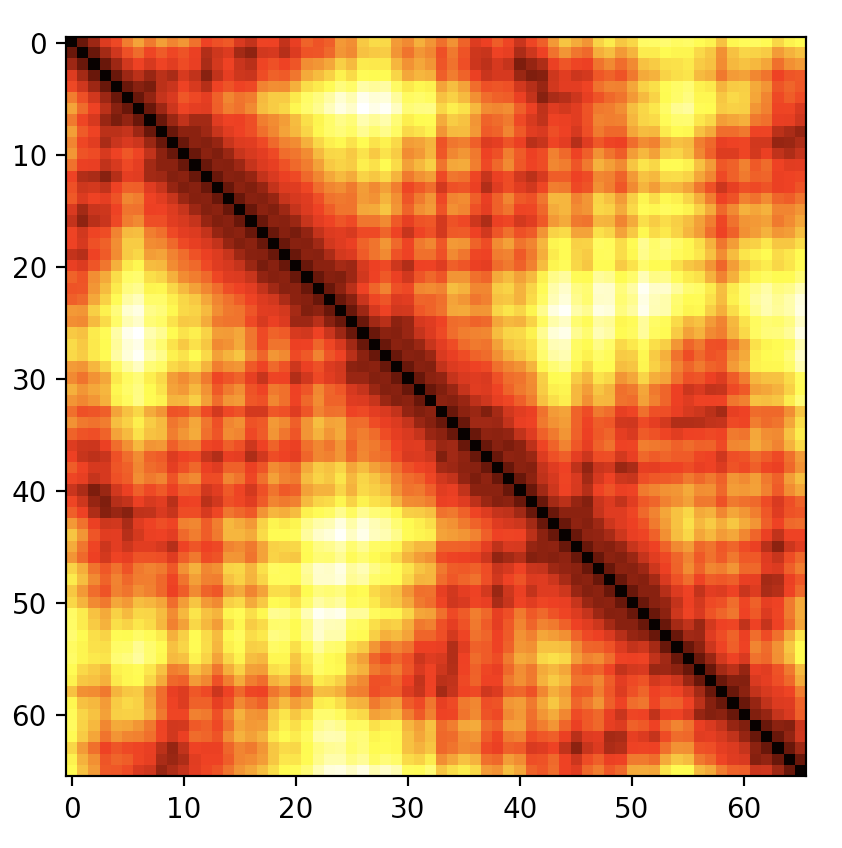
\includegraphics[width=0.3\textwidth]{images/1a8o-ca-plot.png}
\end{latexonly}
\caption{C$\alpha$ distance plot for PDB file 1A8O (HIV capsid C-terminal domain)}
\label{fig:distanceplot}
\end{figure}

\subsubsection{Building a structure from a distance plot}

The all-atom distance plot is another representation of a protein structure, also
invariant to translation and rotation but lacking in chirality information (a
mirror-image structure will generate the same distance plot).  By combining the
distance matrix with the signs of each dihedral angle, it is possible to regenerate
the internal coordinates.  

This work uses equations developed by Blue, the Hedronometer,
discussed in \url{https://math.stackexchange.com/a/49340/409} and further in 
\url{http://daylateanddollarshort.com/mathdocs/Heron-like-Results-for-Tetrahedral-Volume.pdf}.

To begin, we extract the distances and chirality values from `myChain':

%cont-doctest
\begin{minted}{pycon}
>>> # build structure from distance plot:

>>> ## create the all-atom distance plot
>>> distances = myCic.distance_plot()
>>> ## get the signs of the dihedral angles
>>> chirality = myCic.dihedral_signs()
\end{minted}

We need a valid data structure matching `myChain' to correctly rebuild it; using
\texttt{read\_PIC\_seq\(\)} above would work in the general case, but the 1A8O example
used here has some ALTLOC complexity which the sequence alone would not generate.
For demonstration the easiest approach is to simply duplicate the `myChain'
structure, but we set all the atom and internal coordinate chain arrays to 0s
(only for demonstration) just to be certain there is no data coming through from the
original structure:

%cont-doctest
\begin{minted}{pycon}
>>> ## get new, empty data structure : copy data structure from myChain
>>> myChain2 = IC_duplicate(myChain)[0]["A"]
>>> cic2 = myChain2.internal_coord

>>> ## clear the new atomArray and di/hedra value arrays, just for proof
>>> cic2.atomArray = np.zeros((cic2.AAsiz, 4), dtype=np.float64)
>>> cic2.dihedraAngle[:] = 0.0
>>> cic2.hedraAngle[:] = 0.0
>>> cic2.hedraL12[:] = 0.0
>>> cic2.hedraL23[:] = 0.0
\end{minted}

The approach is to regenerate the internal coordinates from the distance plot
data, then generate the atom coordinates from the internal coordinates as shown
above.  To place the final generated structure in the same coordinate space as the
starting structure, we copy just the coordinates for the first three N-C$\alpha$-C
atoms from the chain start of `myChain' to the `myChain2' structure (this is only needed
to demonstrate equivalence at end):

%cont-doctest
\begin{minted}{pycon}
>>> ## copy just the first N-Ca-C coords so structures will superimpose:
>>> cic2.copy_initNCaCs(myChain.internal_coord)
\end{minted}

The \texttt{distance\_to\_internal\_coordinates\(\)} routine needs arrays of the six
inter-atom distances for each dihedron for the target structure.  The convenience
routine \texttt{distplot\_to\_dh\_arrays\(\)} extracts these values from the previously
generated distance matrix as needed, and may be replaced by a user method to
write these data to the arrays in the \texttt{Chain.internal\_coords} object.

%cont-doctest
\begin{minted}{pycon}
>>> ## copy distances to chain arrays:
>>> cic2.distplot_to_dh_arrays(distances)
>>> ## compute angles and dihedral angles from distances:
>>> cic2.distance_to_internal_coordinates(chirality)
\end{minted}

The steps below generate the atom coordinates from the newly generated `myChain2' internal
coordinates, then use the Numpy \texttt{allclose\(\)} routine to confirm that all values match to
better than PDB file resolution:

% this exact test passes on linux as unittest test_rebuild_1a8o, but returns False on linux here!
%xcont-doctest
\begin{minted}{pycon}
>>> ## generate XYZ coordinates from internal coordinates:
>>> myChain2.internal_to_atom_coordinates()
>>> ## confirm result atomArray matches original structure:
>>> np.allclose(cic2.atomArray, myCic.atomArray)
True
\end{minted}

Note that this procedure does not use the entire distance matrix, but only the six local distances
between the four atoms of each dihedral angle.

\subsubsection{Superimposing residues and their neighborhoods}

The \texttt{internal\_coords} module relies on transforming atom coordinates between
different coordinate spaces for both calculation of torsion angles and reconstruction of
structures.  Each dihedron has a coordinate space transform placing its first atom on the
XZ plane, second atom at the origin, and third atom on the +Z axis, as well as a corresponding
reverse transform which will return it to the coordinates in the original structure.  These
transform matrices are available to use as shown below.  By judicious choice of a reference
dihedron, pairwise and higher order residue intereactions can be investigated and visualized
across multiple protein structures, e.g. Figure~\ref{fig:phepairs}.

\begin{figure}[htbp]
\centering
\begin{htmlonly}
\imgsrc[width=360, height=360]{images/phe-pairs-3pbl.png}
\end{htmlonly}
\begin{latexonly}
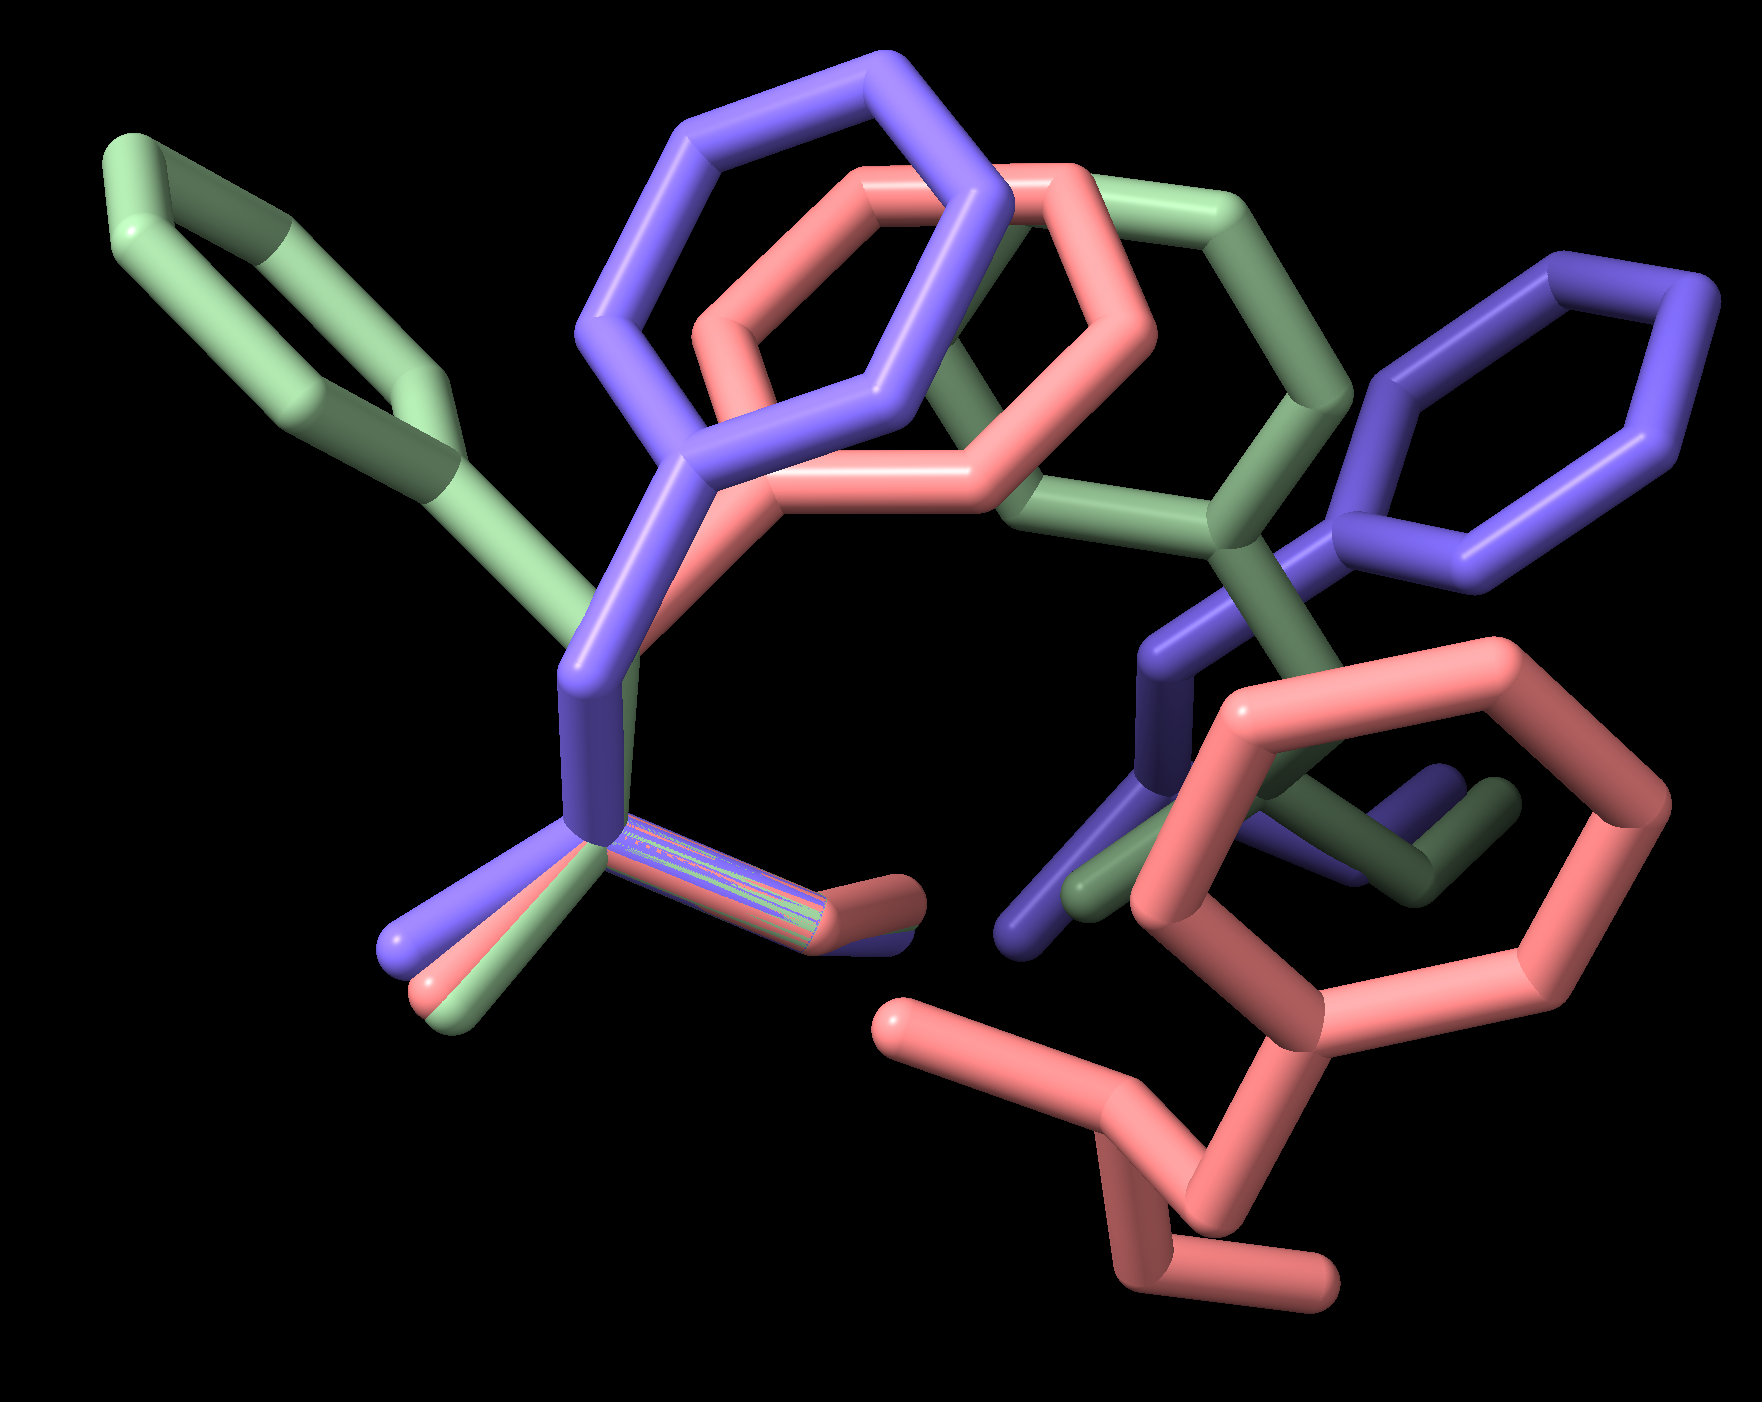
\includegraphics[width=0.7\textwidth]{images/phe-pairs-3pbl.png}
\end{latexonly}
\caption{Neighboring phenylalanine sidechains in PDB file 3PBL (human dopamine D3 receptor)}
\label{fig:phepairs}
\end{figure}
	
This example superimposes each PHE residue in a chain on its N-C$\alpha$-C$\beta$ atoms,
and presents all PHEs in the chain in the respective coordinate space as a simple demonstration.
A more realistic exploration of pairwise sidechain interactions would examine a dataset of
structures and filter for interaction classes as descussed in the relevant literature.

\begin{minted}{python}
# superimpose all phe-phe pairs - quick hack just to demonstrate concept
# for analyzing pairwise residue interactions.  Generates PDB ATOM records
# placing each PHE at origin and showing all other PHEs in environment

## shorthand for key variables:
cic = myChain.internal_coord
resNameNdx = AtomKey.fields.resname
aaNdx = cic.atomArrayIndex

## select just PHE atoms:
pheAtomSelect = [aaNdx.get(k) for k in aaNdx.keys() if k.akl[resNameNdx] == "F"]
aaF = cic.atomArray[pheAtomSelect]  # numpy fancy indexing makes COPY not view

for ric in cic.ordered_aa_ic_list:  # internal_coords version of get_residues()
    if ric.lc == "F":  # if PHE, get transform matrices for chi1 dihedral
        chi1 = ric.pick_angle("chi1")  # N:CA:CB:CG space has C-alpha at origin
        cst = np.transpose(chi1.cst)  # transform TO chi1 space
        # rcst = np.transpose(chi1.rcst)  # transform FROM chi1 space (not needed here)
        cic.atomArray[pheAtomSelect] = aaF.dot(cst)  # transform just the PHEs
        for res in myChain.get_residues():  # print PHEs in new coordinate space
            if res.resname in ["PHE"]:
                print(res.internal_coord.pdb_residue_string())
        cic.atomArray[pheAtomSelect] = aaF  # restore coordinate space from copy
\end{minted}

\subsubsection{3D printing protein structures}

OpenSCAD (\url{https://openscad.org}) is a language for creating solid 3D CAD objects.  
The algorithm to construct a protein structure from internal coordinates is supplied
in OpenSCAD with data describing a structure, such that a model can be generated suitable
for 3D printing.  While other software can generate STL data as a rendering option for
3D printing (e.g. Chimera, \url{https://www.cgl.ucsf.edu/chimera/}), this approach generates
spheres and cylinders as output and is therefore more amenable to modifications relevant to
3D printing protein structures.  Individual residues and bonds can be selected
in the OpenSCAD code for special handling, such as highlighting by size or adding
rotatable bonds in specific positions (see \url{https://www.thingiverse.com/thing:3957471}
for an example).

\begin{minted}{python}
# write OpenSCAD program of spheres and cylinders to 3d print myChain backbone
## set atom load filter to accept backbone only:
IC_Residue.accept_atoms = IC_Residue.accept_backbone
## set chain break cutoff very high to bridge missing residues with long bonds
IC_Chain.MaxPeptideBond = 4.0
## delete existing data to force re-read of all atoms with attributes set above:
myChain.internal_coord = None
write_SCAD(myChain, "myChain.scad", scale=10.0)
\end{minted}

\subsubsection{\texttt{internal\_coords} control attributes}

A few control attributes are available in the \texttt{internal\_coords} classes to modify or
filter data as internal coordinates are calculated.  These are listed in Table~\ref{table:ic-attribs}:

\begin{table}
	\begin{tabular}{|l|l|l|l|}
		\hline
		Class&Attribute&Default&Effect\\
		\hline
		\hline
		AtomKey& d2h&False&Convert D atoms to H if True\\
		\hline
		IC\_Chain&MaxPeptideBond&1.4&Max C-N length w/o chain break; make large to link over missing residues for 3D models \\
		\hline
		IC\_Residue&accept\_atoms&mainchain, hydrogen atoms&override to remove some or all sidechains, H's, D's\\
		\hline
		&accept\_resnames&CYG, YCM, UNK&3-letter names for HETATMs to process, backbone only unless added to ic\_data.py \\
		\hline
		&gly\_Cbeta&False&override to generate Gly C$\beta$ atoms based on database averages \\
		\hline
	\end{tabular}
	\caption{Control attributes in Bio.PDB.internal\_coords.}
	\label{table:ic-attribs}
\end{table}

\subsection{Determining atom-atom contacts}

Use \texttt{NeighborSearch} to perform neighbor lookup.
The neighbor lookup is done using a KD tree module written in C (see the \texttt{KDTree} class in module \texttt{Bio.PDB.kdtrees}), making it very fast.
It also includes a fast method to find all point pairs within a certain distance of each other.

\subsection{Superimposing two structures}

Use a \texttt{Superimposer} object to superimpose two coordinate sets.
This object calculates the rotation and translation matrix that rotates
two lists of atoms on top of each other in such a way that their RMSD
is minimized. Of course, the two lists need to contain the same number
of atoms. The \texttt{Superimposer} object can also apply the rotation/translation
to a list of atoms. The rotation and translation are stored as a tuple
in the \texttt{rotran} attribute of the \texttt{Superimposer} object
(note that the rotation is right multiplying!). The RMSD is stored
in the \texttt{rmsd} attribute.

The algorithm used by \texttt{Superimposer} comes from \cite[Golub \& Van Loan]{golub1989} and makes use of singular value decomposition (this is implemented in the general \texttt{Bio.SVDSuperimposer} module).

Example:

\begin{minted}{pycon}
>>> sup = Superimposer()
# Specify the atom lists
# 'fixed' and 'moving' are lists of Atom objects
# The moving atoms will be put on the fixed atoms
>>> sup.set_atoms(fixed, moving)
# Print rotation/translation/rmsd
>>> print(sup.rotran)
>>> print(sup.rms)
# Apply rotation/translation to the moving atoms
>>> sup.apply(moving)
\end{minted}

To superimpose two structures based on their active sites, use the active site atoms to calculate the rotation/translation matrices (as above), and apply these to the whole molecule.

\subsection{Mapping the residues of two related structures onto each other}

First, create an alignment file in FASTA format, then use the \texttt{StructureAlignment}
class. This class can also be used for alignments with more than two
structures.

\subsection{Calculating the Half Sphere Exposure}

Half Sphere Exposure (HSE) is a new, 2D measure of solvent exposure
\cite{hamelryck2005}.
Basically, it counts the number of C$\alpha$ atoms around a residue
in the direction of its side chain, and in the opposite direction
(within a radius of $13 \AA$). Despite its simplicity, it outperforms
many other measures of solvent exposure.

HSE comes in two flavors: HSE$\alpha$ and HSE$\beta$. The former
only uses the C$\alpha$ atom positions, while the latter uses the
C$\alpha$ and C$\beta$ atom positions. The HSE measure is calculated
by the \texttt{HSExposure} class, which can also calculate the contact
number. The latter class has methods which return dictionaries that
map a \texttt{Residue} object to its corresponding HSE$\alpha$, HSE$\beta$
and contact number values.

Example:

\begin{minted}{pycon}
>>> model = structure[0]
>>> hse = HSExposure()
# Calculate HSEalpha
>>> exp_ca = hse.calc_hs_exposure(model, option="CA3")
# Calculate HSEbeta
>>> exp_cb = hse.calc_hs_exposure(model, option="CB")
# Calculate classical coordination number
>>> exp_fs = hse.calc_fs_exposure(model)
# Print HSEalpha for a residue
>>> print(exp_ca[some_residue])
\end{minted}

\subsection{Determining the secondary structure}

For this functionality, you need to install DSSP (and obtain a license
for it --- free for academic use, see \url{https://swift.cmbi.umcn.nl/gv/dssp/}).
Then use the \texttt{DSSP} class, which maps \texttt{Residue} objects
to their secondary structure (and accessible surface area). The DSSP
codes are listed in Table~\ref{table:DSSP-codes}. Note that DSSP (the
program, and thus by consequence the class) cannot handle multiple
models!

\begin{table}
\begin{tabular}{|c|c|}
\hline
Code&
Secondary structure \\
\hline
\hline
H&
$\alpha$-helix \\
\hline
B&
Isolated $\beta$-bridge residue \\
\hline
E&
Strand \\
\hline
G&
3-10 helix \\
\hline
I&
$\Pi$-helix \\
\hline
T&
Turn\\
\hline
S&
Bend \\
\hline
-&
Other\\
\hline
\end{tabular}
\caption{DSSP codes in Bio.PDB.}
\label{table:DSSP-codes}
\end{table}

The \texttt{DSSP} class can also be used to calculate the accessible surface area of a residue. But see also section \ref{sec:residue_depth}.

\subsection{Calculating the residue depth}
\label{sec:residue_depth}

Residue depth is the average distance of a residue's atoms from the
solvent accessible surface. It's a fairly new and very powerful parameterization
of solvent accessibility. For this functionality, you need to install
Michel Sanner's MSMS program (\url{https://www.scripps.edu/sanner/html/msms_home.html}).
Then use the \texttt{ResidueDepth} class. This class behaves as a
dictionary which maps \texttt{Residue} objects to corresponding (residue
depth, C$\alpha$ depth) tuples. The C$\alpha$ depth is the distance
of a residue's C$\alpha$ atom to the solvent accessible surface.

Example:

\begin{minted}{pycon}
>>> model = structure[0]
>>> rd = ResidueDepth(model, pdb_file)
>>> residue_depth, ca_depth = rd[some_residue]
\end{minted}
You can also get access to the molecular surface itself (via the \texttt{get\_surface}
function), in the form of a Numeric Python array with the surface points.

\section{Common problems in PDB files}

It is well known that many PDB files contain semantic errors (not the
structures themselves, but their representation in PDB files).
Bio.PDB tries to handle this in two ways. The PDBParser
object can behave in two ways: a restrictive way and a permissive
way, which is the default.

Example:

\begin{minted}{pycon}
# Permissive parser
>>> parser = PDBParser(PERMISSIVE=1)
>>> parser = PDBParser()  # The same (default)
# Strict parser
>>> strict_parser = PDBParser(PERMISSIVE=0)
\end{minted}
In the permissive state (DEFAULT), PDB files that obviously contain
errors are ``corrected'' (i.e. some residues or atoms are left out).
These errors include:

\begin{itemize}
\item Multiple residues with the same identifier
\item Multiple atoms with the same identifier (taking into account the altloc
identifier)
\end{itemize}
These errors indicate real problems in the PDB file (for details see
\cite[Hamelryck and Manderick, 2003]{hamelryck2003a}). In the restrictive state, PDB files with errors cause an exception to occur. This is useful to find errors in PDB files.

Some errors however are automatically corrected. Normally each disordered
atom should have a non-blank altloc identifier. However, there are
many structures that do not follow this convention, and have a blank
and a non-blank identifier for two disordered positions of the same
atom. This is automatically interpreted in the right way.

Sometimes a structure contains a list of residues belonging to chain
A, followed by residues belonging to chain B, and again followed by
residues belonging to chain A, i.e. the chains are 'broken'. This
is also correctly interpreted.

\subsection{Examples}
\label{sec:problem_structures}

The PDBParser/Structure class was tested on about 800 structures (each belonging
to a unique SCOP superfamily). This takes about 20 minutes, or on average 1.5
seconds per structure. Parsing the structure of the large ribosomal subunit
(1FKK), which contains about 64000 atoms, takes 10 seconds on a 1000 MHz PC.

Three exceptions were generated in cases where an unambiguous data structure
could not be built. In all three cases, the likely cause is an error in the
PDB file that should be corrected. Generating an exception in these cases
is much better than running the chance of incorrectly describing
the structure in a data structure.

\subsubsection{Duplicate residues}

One structure contains two amino acid residues in one chain with the same sequence
identifier (resseq 3) and icode. Upon inspection it was found that this chain
contains the residues Thr A3, \ldots, Gly A202, Leu A3, Glu A204. Clearly,
Leu A3 should be Leu A203. A couple of similar situations exist for structure
1FFK (which e.g. contains Gly B64, Met B65, Glu B65, Thr B67, i.e. residue Glu
B65 should be Glu B66).

\subsubsection{Duplicate atoms}

Structure 1EJG contains a Ser/Pro point mutation in chain A at position 22.
In turn, Ser 22 contains some disordered atoms. As expected, all atoms belonging
to Ser 22 have a non-blank altloc specifier (B or C). All atoms of Pro 22 have
altloc A, except the N atom which has a blank altloc. This generates an exception,
because all atoms belonging to two residues at a point mutation should have
non-blank altloc. It turns out that this atom is probably shared by Ser and
Pro 22, as Ser 22 misses the N atom. Again, this points to a problem in the
file: the N atom should be present in both the Ser and the Pro residue, in both
cases associated with a suitable altloc identifier.

\subsection{Automatic correction}

Some errors are quite common and can be easily corrected without much risk of
making a wrong interpretation. These cases are listed below.

\subsubsection{A blank altloc for a disordered atom}

Normally each disordered atom should have a non-blank altloc identifier. However,
there are many structures that do not follow this convention, and have a blank
and a non-blank identifier for two disordered positions of the same atom. This
is automatically interpreted in the right way.

\subsubsection{Broken chains}

Sometimes a structure contains a list of residues belonging to chain A, followed
by residues belonging to chain B, and again followed by residues belonging to
chain A, i.e. the chains are ``broken''. This is correctly interpreted.

\subsection{Fatal errors}

Sometimes a PDB file cannot be unambiguously interpreted. Rather than guessing
and risking a mistake, an exception is generated, and the user is expected to
correct the PDB file. These cases are listed below.

\subsubsection{Duplicate residues}

All residues in a chain should have a unique id. This id is generated based
on:

\begin{itemize}
\item The sequence identifier (resseq).
\item The insertion code (icode).
\item The hetfield string (``W'' for waters and ``H\_'' followed by the
residue name for other hetero residues)
\item The residue names of the residues in the case of point mutations (to store the
Residue objects in a DisorderedResidue object).
\end{itemize}
If this does not lead to a unique id something is quite likely wrong, and an
exception is generated.

\subsubsection{Duplicate atoms}

All atoms in a residue should have a unique id. This id is generated based on:

\begin{itemize}
\item The atom name (without spaces, or with spaces if a problem arises).
\item The altloc specifier.
\end{itemize}
If this does not lead to a unique id something is quite likely wrong, and an
exception is generated.

\section{Accessing the Protein Data Bank}

\subsection{Downloading structures from the Protein Data Bank}

Structures can be downloaded from the PDB (Protein Data Bank)
by using the \texttt{retrieve\_pdb\_file} method on a \texttt{PDBList} object.
The argument for this method is the PDB identifier of the structure.

\begin{minted}{pycon}
>>> pdbl = PDBList()
>>> pdbl.retrieve_pdb_file("1FAT")
\end{minted}

The \texttt{PDBList} class can also be used as a command-line tool:
\begin{minted}{pycon}
python PDBList.py 1fat
\end{minted}
The downloaded file will be called \texttt{pdb1fat.ent} and stored
in the current working directory. Note that the \texttt{retrieve\_pdb\_file}
method also has an optional argument \texttt{pdir} that specifies
a specific directory in which to store the downloaded PDB files.

The \texttt{retrieve\_pdb\_file} method also has some options to specify
the compression format used for the download, and the program used
for local decompression (default \texttt{.Z} format and \texttt{gunzip}).
In addition, the PDB ftp site can be specified upon creation of the
\texttt{PDBList} object. By default, the server of the Worldwide Protein Data Bank (\url{ftp://ftp.wwpdb.org/pub/pdb/data/structures/divided/pdb/})
is used. See the API documentation for more details. Thanks again
to Kristian Rother for donating this module.

\subsection{Downloading the entire PDB}

The following commands will store all PDB files in the \texttt{/data/pdb}
directory:

\begin{minted}{pycon}
python PDBList.py all /data/pdb

python PDBList.py all /data/pdb -d
\end{minted}
\noindent The API method for this is called \texttt{download\_entire\_pdb}.
Adding the \texttt{-d} option will store all files in the same directory.
Otherwise, they are sorted into PDB-style subdirectories according
to their PDB ID's. Depending on the traffic, a complete download will
take 2-4 days.

\subsection{Keeping a local copy of the PDB up to date}

This can also be done using the \texttt{PDBList} object. One simply
creates a \texttt{PDBList} object (specifying the directory where
the local copy of the PDB is present) and calls the \texttt{update\_pdb}
method:

\begin{minted}{pycon}
>>> pl = PDBList(pdb="/data/pdb")
>>> pl.update_pdb()
\end{minted}
One can of course make a weekly \texttt{cronjob} out of this to keep
the local copy automatically up-to-date. The PDB ftp site can also
be specified (see API documentation).

\texttt{PDBList} has some additional methods that can be of use. The
\texttt{get\_all\_obsolete} method can be used to get a list of all
obsolete PDB entries. The \texttt{changed\_this\_week} method can
be used to obtain the entries that were added, modified or obsoleted
during the current week. For more info on the possibilities of \texttt{PDBList},
see the API documentation.

\section{General questions}

\subsection{How well tested is Bio.PDB?}

Pretty well, actually. Bio.PDB has been extensively tested on nearly
5500 structures from the PDB - all structures seemed to be parsed
correctly. More details can be found in the Bio.PDB Bioinformatics
article. Bio.PDB has been used/is being used in many research projects
as a reliable tool. In fact, I'm using Bio.PDB almost daily for research
purposes and continue working on improving it and adding new features.

\subsection{How fast is it?}

The \texttt{PDBParser} performance was tested on about 800 structures
(each belonging to a unique SCOP superfamily). This takes about 20
minutes, or on average 1.5 seconds per structure. Parsing the structure
of the large ribosomal subunit (1FKK), which contains about 64000
atoms, takes 10 seconds on a 1000 MHz PC. In short: it's more than
fast enough for many applications.

\subsection{Is there support for molecular graphics?}

Not directly, mostly since there are quite a few Python based/Python
aware solutions already, that can potentially be used with Bio.PDB.
My choice is Pymol, BTW (I've used this successfully with Bio.PDB,
and there will probably be specific PyMol modules in Bio.PDB soon/some
day). Python based/aware molecular graphics solutions include:

\begin{itemize}
\item PyMol: \url{https://pymol.org/}
\item Chimera: \url{https://www.cgl.ucsf.edu/chimera/}
\item PMV: \url{http://www.scripps.edu/~sanner/python/}
\item Coot: \url{https://www2.mrc-lmb.cam.ac.uk/personal/pemsley/coot/}
\item CCP4mg: \url{http://www.ccp4.ac.uk/MG/}
\item mmLib: \url{http://pymmlib.sourceforge.net/}
\item VMD: \url{https://www.ks.uiuc.edu/Research/vmd/}
\item MMTK: \url{http://dirac.cnrs-orleans.fr/MMTK/}
\end{itemize}

\subsection{Who's using Bio.PDB?}

Bio.PDB was used in the construction of DISEMBL, a web server that
predicts disordered regions in proteins (\url{http://dis.embl.de/}). Bio.PDB has also been used to
perform a large scale search for active sites similarities between
protein structures in the PDB \cite[Hamelryck, 2003]{hamelryck2003b}, and to develop a new algorithm
that identifies linear secondary structure elements \cite[Majumdar \textit{et al.}, 2005]{majumdar2005}.

Judging from requests for features and information, Bio.PDB is also
used by several LPCs (Large Pharmaceutical Companies :-).

% Perhaps this section should be updated for other Biopython modules, and
% moved to the Biopython FAQ above.
